\chapter{Appendix A:  BrowserAudit, the previous versions}

\section{Initial project (V1)}

Charlie Hothersall's thesis can be found in \cite{charlie} , Browseraudit was built largely as a modification of Mocha with Chai assertion library \
Mocha was meant to be a nodejs testing library, but had browser support, hence allowed to have a base framework to save time and get the actual tests written \

It was really thought of as a Unit Testing framework code running on the browser which was in a way a valid analogy to Unit tests that the browser developers would \
have written for the implementation of security policies for their browsers, but of course here done at the client level. While Mocha helped save some time for the task and
it's asynchronous options were appreciated to save time running the tests; It did however need to be heavily customized with a rebuilt frontend using a Reporter interface that \
triggers callbacks on testStart end and Suite start and End.\ 

The frontend was beautifully done, making use of twitter bootstrap, with suitable design that didn't get in the way of understanding the tests, and that offered expandable\
information about the tests from just the name and category and Pass/fail down to the exact code and the assertions that fail or errors matching different users capabilities.\

There were a fair amount of basic tests of which the most notable one that illustrates an important tool for running these tests which is the img src property:
you can see this in action in \ref{fig:sop} 

\begin{figure}
\centering
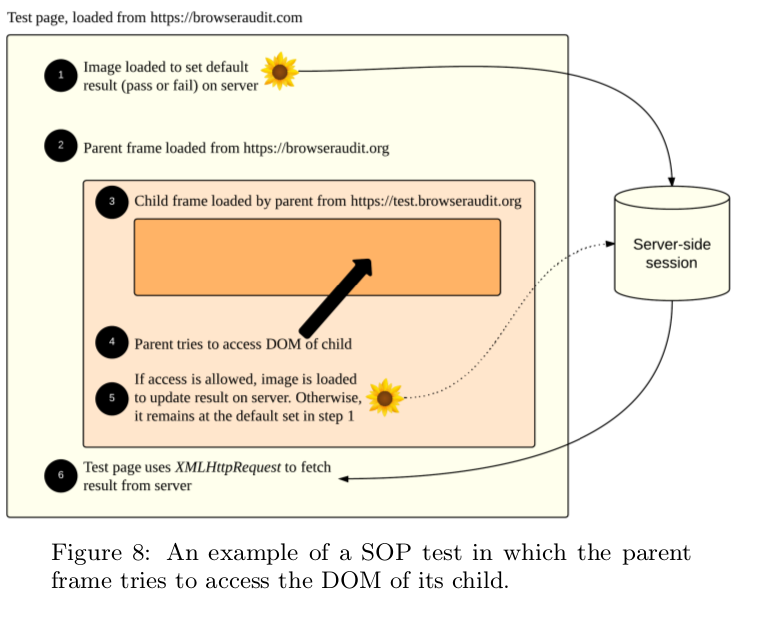
\includegraphics[width=1\textwidth]{./SOPbasic.png}
\caption{\label{fig:sop}Same origin policy typical test}
\end{figure}

As you can see the mechanism of img src property is used to communicate to the server on predefined appropriate pass/fail testiD endpoints. This is because 
the img object is not subject to any limitations and doesn't interfere in the testing of the security policy itself. This is used in many other types of tests.

The initial version had over 300 test tests and by using plain javascript and dilligently avoiding methods that are not adopted by most browsers,
The initial browseraudit version was supported and tested on these browsers:

\begin{itemize}
 \item Firefox desktop version 26, 29:  4 /306 and 6/306 failures respectively
 \item Android version 30: 14 failures
 \item Ie10: 74/306 failures issues running the actual tests, the failures are test implementation issues.
 \item Ie11: 64/306 In this instance some of the tests that failed in ie10 run but they are still failures.
 \item Safari Desktop version 6 and Ios Version: 6 /286 runs fast with few errors, less tests because no HSTS.
 \item Android 4.2.2: 64/267 problems with CORS and AJAX implementation
 \item Android 4.4.2: 2/286 failing test due to X-frame-Options ALLOW FROM not implemented.
\end{itemize}

Most notable discoveries of browseraudit were firefox's CSP implementation: CSP allows local CSS @import with only `unsafe-inline' set and 
CSP allows local Worker construction with only `unsafe-inline' set a very good spot that would have been very hard to detect in the wild!

\section{Current version (V2)}

Dr Sergio maffeis and Chris Novakovic took the project in hand and improved coverage drastically, there are now up to 404 tests and counting.
Matching the newer CSP standard, clickjacking and framebustig related tests etc..

The fact that Mocha was a nodejs package that had browser support started to show, because browser coverage is not terrific with the test framework.
Everybody had forgotten ie6 but ie8+ is considered a modern browser by many and we aim to be able to test any configuration in the wild, and ie at the time
of writing still represents 25+\% of the marketshare.\

For this reason the team decided to go for its own test framework. which greatly simplifies the whole application, avoiding all the boiletplate that \
turned a unit testing framework with browser support into a browser testing framework.

This current version , which we will refer to as (V2) is constantly being upgraded, and close integration with the code is required for my implementation\
but the new tiered architecture is striving towards a simpler, more modular way to deal with the tests which we will describe in the rest of this section. 

There is an intermediate version, V1.5, if you will, which was still running mocha and chai for test running but had all the extra tests written and \
was in the draft version of the browseraudit paper , available at \cite{maffeis}. We will only focus on the latest version because the framework and tests\
are thoroughly described in \cite{charlie}.

You can see screenshots of the latest version's home screen in \ref{fig:mainscreen} and expanded test category in \ref{fig:testresult}.


\begin{figure}
\centering
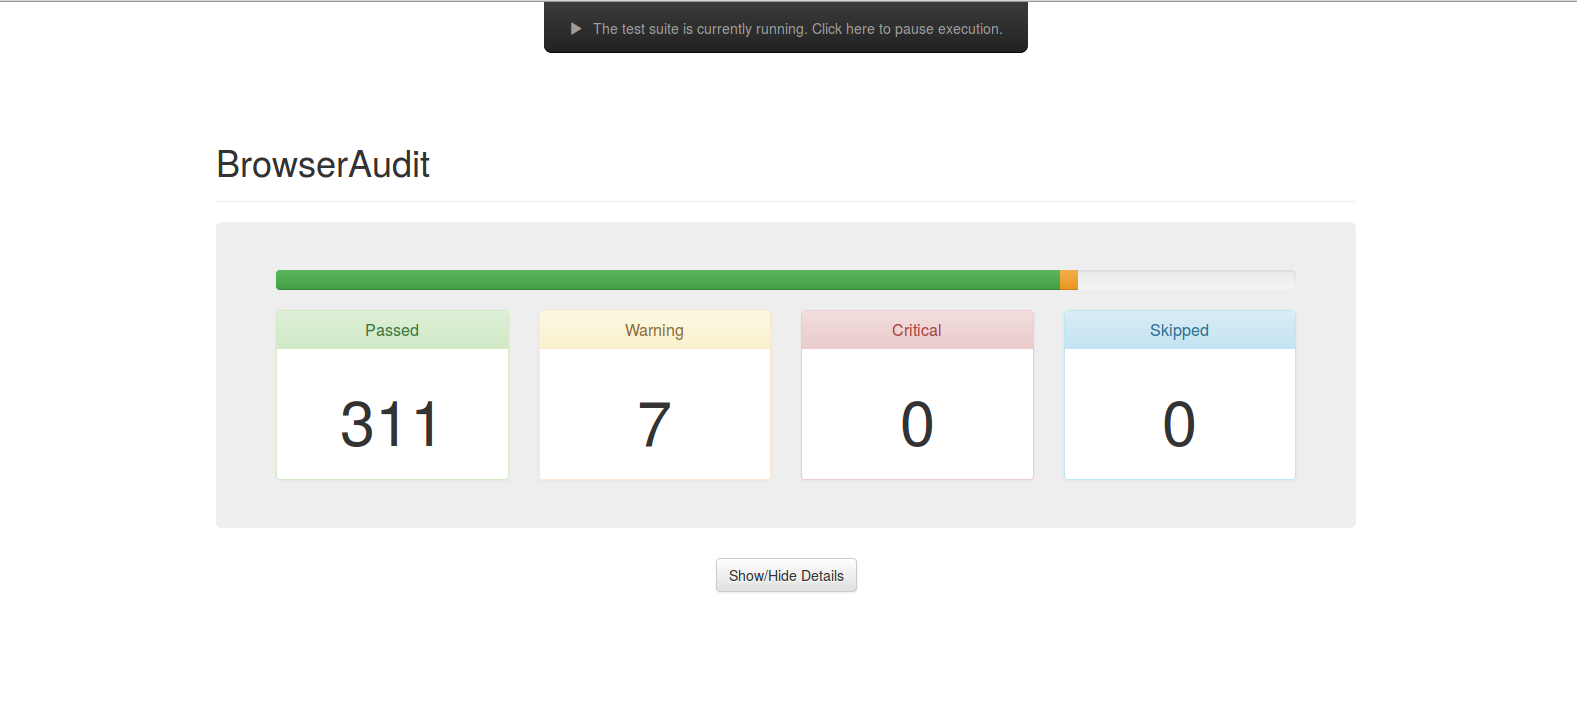
\includegraphics[width=1\textwidth]{./browser20.png}
\caption{\label{fig:mainscreen}BrowserAudit 2 running tests}
\end{figure}

\begin{figure}
\centering
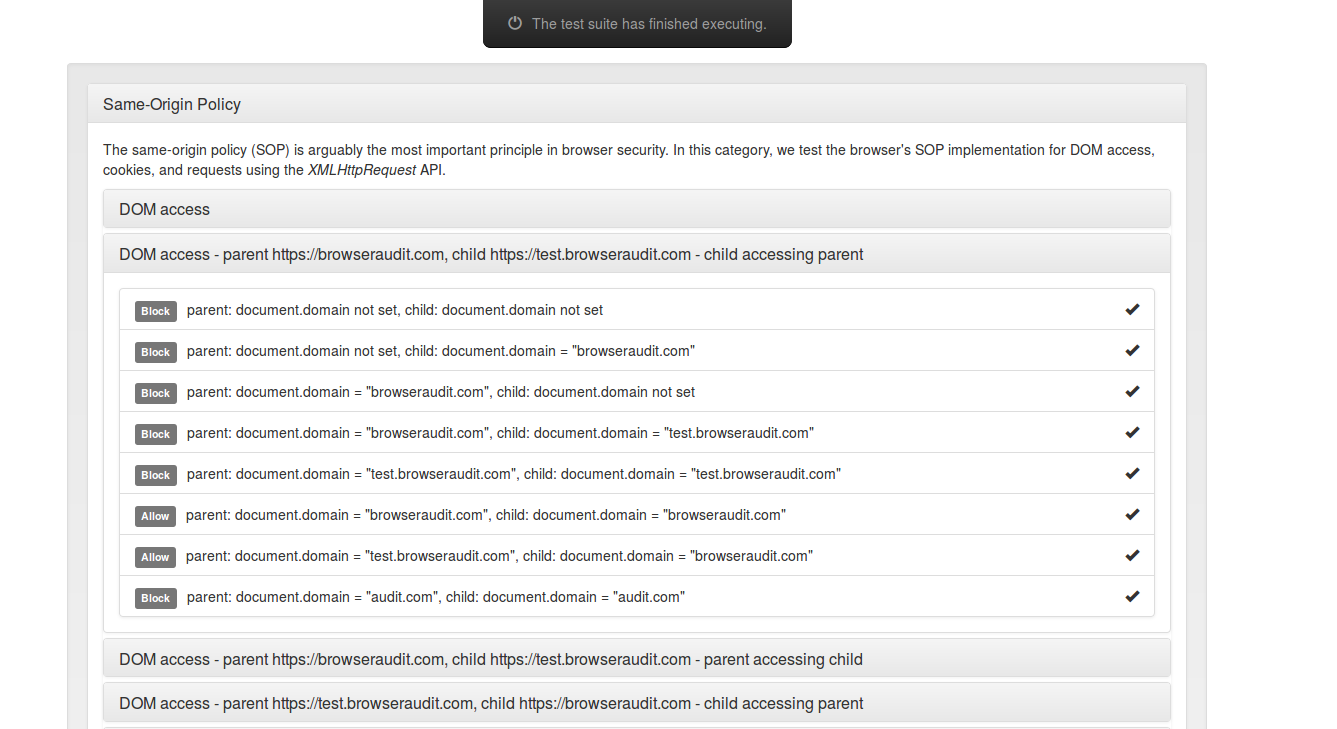
\includegraphics[width=1\textwidth]{./browsertest.png}
\caption{\label{fig:testresult}BrowserAudit tests finished}
\end{figure}

\subsection{Test Backend in V2}

\subsubsection{Overall working principle}
\label{label:workprinc}

Under the current version, categories, testsuites and tests are loaded from a postgres database, and test results "objects" are also saved on the database.
This is a Backend centric architecture which writes js hooks to the frontend.. the execution object models are loaded onto go code which generate javascript on the fly.

If a test is live, the appropriate javascript is included, calling bridge functions that look like addcategory(foo,bar,..) or addTest(jah,jah) registering different 
categories and tests, it also passes their function invocation code to client test template functions if needed with the correct html structures hardcoded as static assets.

This leaves to the frontend the sole mission to execute the code and update the UI with appropriate categories, descriptions, test suites, expected test outcomes
and actual outcomes. Due to different policies often requiring different headers or behaviour from the server the client code for a particular category is tied to server 
endpoints, this is explained in \ref{label:servercode}.

It is also worthwhile to note that the go server has the task of saving the test results correctly to the database but this is done in one go at the end of execution of tests\
and it's is the client test execution framework that generates the required data, which is 
flexible because it would save tests results from tests that were not loaded from the go server for example. see \ref{subsec:reporter}.

\subsubsection{PostgreSQL model}

Take the time to check \ref{fig:model} the foreign keys have been conveniently marked with a diamond connector, we did not go into the details of suite execution settings.
because it was containing identical data in terms of displaymode this is a yet unused provision for future test suite display options among other settings.

As you can see there is a clear distinction to make between tests which belong to catgories and executions of browserAudit on users machines and the outcome of tests\
during those executions. This follows what was explained earlier about the execution model. \

As you can see almost everything about the tests is stored in database, except the function it's calling itself , which for now is hardcoded onto the client side\
into the testtemplates.js file, which means there is high coupling between the test database model and the client side invokers. 
Although at present it is manageable, In order to make the system extensible, modular and ultimately less fragile, we'll need to find a way to work around this
to extend browseraudit.
Once again to be clear, the test categories are fixed, and the way categories and tests are currently being added is manually to the database 
and this is manageable since the tests are added progressively, but the first step we wil take is to improve on this and make a test management interface, see \ref{label:addtest}.


\begin{figure}
\centering
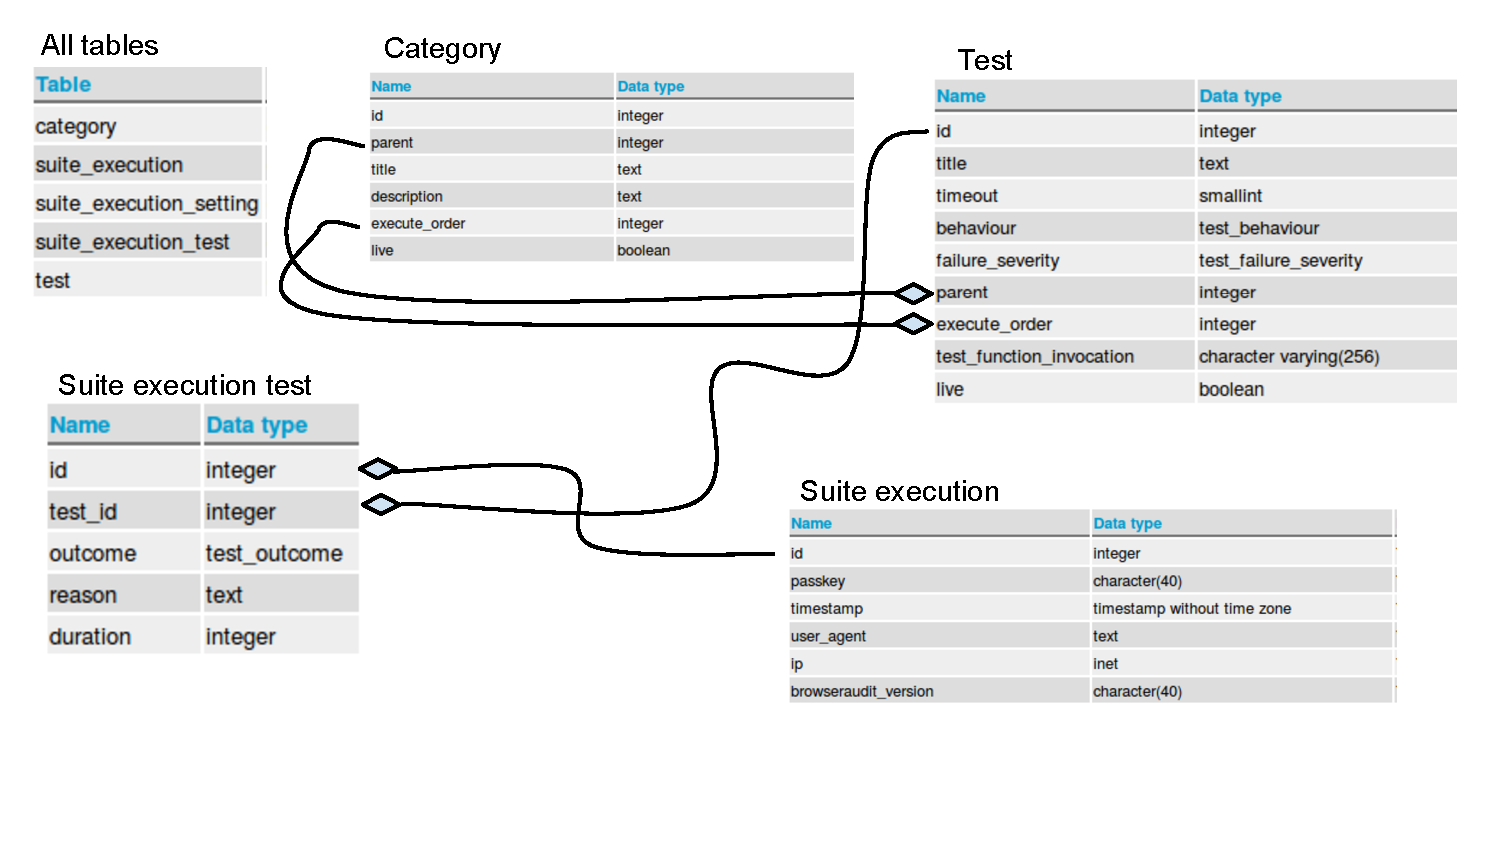
\includegraphics[width=1\textwidth]{db.pdf}
\caption{\label{fig:model}Database description of most important tables.}
\end{figure}


\subsubsection{The server}

\emph{Nginx}

There is an Nginx reverse proxy serving the static content and caching where cache directives are to allow caching for a response. this is thoroughly explained both in 
\cite{charlie} and \cite{maffeis}. 

\emph{the Go server}

\label{label:servercode}

As explained in the Overall execution model in \ref{label:workprinc}, the server main roles are:
\begin{itemize}
 \item generating the script file containing all the tests in the database. 
 \item Providing endpoints that respond to requests in ways that are needed to test the policies. 
 \item handling the pages that are not cacheable ie index.
 \item Receiving the results and saving them to the database.
\end{itemize}

Remember that what is actually saved in the database in terms of test execution is the invocation of the right client template (javascript) function with
suitable parameters and identification for later logging of results.
We will now go into the details of the client code generation that handles those classes of tests in section \ref{subsec:client}.

The other interesting role to expand on is the Go server handling of the responses at the appropriate endpoints for the types or categories of tests;

For example, we will walkthrough all aspects of handling CSP tests, in particular the server side code that enables the cspTest client test template function:

\begin{verbatim}

r.HandleFunc("/csp/pass/{id:[0-9]+}/{file:[a-z0-9-]+}", CSPPassHandler)

\end{verbatim}

this CSPPassHandler would be defined in a seperate go module file, csp.go which has the function below and others like CSPServeFile that we will not show here:

\begin{verbatim}
 func CSPPassHandler(w http.ResponseWriter, r *http.Request) {
	r.ParseForm()
	addManualCookie(r)
	session, _ := store.Get(r, "browseraudit")

	id := mux.Vars(r)["id"]
	session.Values["csp"+id] = "pass"
	session.Save(r, w)
	fmt.Println("Recording PASS for CSP test " + id)

	CSPServeFile(w, r)
}
\end{verbatim}

the tests can be pretty specific in what it requires the server to do and this is why there are so many modules dealing with different policies,
it is unclear how this can be made generic, unfortunately this also burdens our potential design for extensibility with perhaps the extra task of writing
go functions to deal with any potential new categories we come up with in case we pursue such an extension of browseraudit.
But in case we don't need any new behaviour from the server our test reporting interface automatically handles reporting for a client side test. 
we will describe the reporting interface in \ref{subsec:reporter}.

We mentioned that the go server creates a javascript file containing calls to test suite methods addcategory and addtest with the appropriate parameters stored in database
here is a couple examples from the file:
\begin{verbatim}

filename:  (categoryid) 1,2, 3 ...  ?_=1432914480170 (execution id) .js

// Automatically-generated BrowserAudit test suite


browserAuditTestFramework.addCategory(1, null, "Same-Origin Policy", 
"<p>The same-origin policy (SOP) is arguably the most important principle in browser security. 
In this category, we test the browser's SOP implementation for DOM access, cookies, and requests    
using the <em>XMLHttpRequest</em> API.</p>");	// adding a category

browserAuditTestFramework.addTest(1, 2,
"child https://browseraudit.com accessing parent https://browseraudit.org", 
"block", null, // this time a test calling the parentChildSopTest client test template function
parentChildSopTest(1, true, false, "https://browseraudit.org", "none", "https://browseraudit.com", "none")); 


browserAuditTestFramework.addTest(2, 2, "parent https://browseraudit.com accessing child https://browseraudit.org", "block", null, parentChildSopTest(2, true, true, "https://browseraudit.com", "none", "https://browseraudit.org", "none"));
 
\end{verbatim}

\subsubsection{The Client test classes}
\label{subsec:client}

The client test classes are shown in the following table with the literal function names and short description \
these are the methods called by the tests that are in the database:

\begin{itemize}
 \item parentChildSopTest // Same-Origin Policy -> DOM access
 \item ajaxSopTest // Same-Origin Policy -> XMLHttpRequest
 \item domainScopeCookieTest // Same-Origin Policy -> Cookies - domain scope
 \item cookiePathScope // Same-Origin Policy -> Cookies - path scope
 \item cspTest //Content Security Policy
 \item originExpect // Cross-Origin Resource Sharing -> Access-Control-Allow-Origin  
 \item methodExpect // Cross-Origin Resource Sharing -> Access-Control-Allow-Methods
 \item headersExpect// Cross-Origin Resource Sharing -> Access-Control-Allow-Headers
 \item exposeExpect // Cross-Origin Resource Sharing -> Access-Control-Expose-Headers
 \item cookiesHttpOnlyServerToScript // Cookies -> HttpOnly flag -> HTTP-only cookie set by server and accessed from JavaScript
 \item cookiesHttpOnlyScriptToServer  // Cookies -> HttpOnly flag -> HTTP-only cookie set by JavaScript (should not be sent to server)
 \item cookiesSecureServerToScriptHTTPS // Cookies -> Secure flag -> cookie set by server should be sent over HTTPS
 \item cookiesSecureScriptToServerHTTP // Cookies -> Secure flag -> cookie set by JavaScript should not be sent over HTTP
 \item requestRefererHTTPSToHTTP // Request Headers -> Referer -> should not be sent over non-secure request if the referring page was transferred with a secure protocol
 \item frameOptionsTest // Response Headers -> X-Frame-Options
 \item hstsTest // Response Headers -> Strict-Transport-Security
\end{itemize}

This interface is a necessary evil, and as explained in the previous section one of the aims of this project is to try to make this
more usable in order to clean up the interface and generalise tests as much as possible.


\subsubsection{Test Reporting}
\label{subsec:reporter}

After all tests are finished the test execution framework sends the full report to the server by first calling  $$"/suite__execution/put"$$
which calls PutSuiteExecutionHandler. This function populates the below structs and writes the query to db appropriately.
The structure is self-explanatory, this is registering an execution of browseraudit to which test executions will refer to it.

\begin{verbatim}

type SuiteExecution struct {
	Id                  int                   `json:"id"`
	Passkey             string                `json:"passkey"`
	Timestamp           time.Time             `json:"timestamp"`
	UserAgent           string                `json:"userAgent"`
	IP                  string                `json:"ip"`
	BrowserAuditVersion string                `json:"browserAuditVersion"`
	Settings            map[string]string     `json:"settings"`
	TestResults         map[string]TestResult `json:"testResults"`
}

\end{verbatim}

When all tests finish successive calls to $$"/suite_execution/get/{id:[0-9]+}/{passkey:[0-9a-f]+}"$$ calls GetSuiteExecutionHandler.

GetSuiteExecutionHandler creates records for individual test Outcomes, the primary key Id refers to the id of a test execution
inserted through the PUT interface described above. testId ASK CHRIS ABOUT THIS. 

\begin{verbatim}

type SuiteExecutionHierarchyRow struct {
	Type                   string         `db:"type"`
	Id                     int            `db:"id"`
	Title                  string         `db:"title"`
	Description            sql.NullString `db:"description"`
	Behaviour              sql.NullString `db:"behaviour"`
	TestFunctionInvocation sql.NullString `db:"test_function_invocation"`
	Timeout                sql.NullInt64  `db:"timeout"`
	Parent                 sql.NullInt64  `db:"parent"`
	OutcomeTotal           NullIntSlice   `db:"outcome_total"`
	Outcome                sql.NullString `db:"outcome"`
	Reason                 sql.NullString `db:"reason"`
	Duration               sql.NullInt64  `db:"duration"`
}

\end{verbatim}


